\documentclass{beamer}
\usetheme{CambridgeUS}
\title[Process]{The Koopman operator identification algorithm}
\subtitle{Nonlinear MPC over the Van Der Pol oscillator}
\institute[Polimi]{Politecnico di Milano}
\author{Sergio Vanegas}
\date{\today}

\usepackage{listings}
\usepackage[framed,numbered,autolinebreaks,useliterate]{mcode/mcode}

\usepackage{caption}
\usepackage{subcaption}
\usepackage{dirtytalk}

\usepackage{graphicx}

\usepackage{siunitx}


\begin{document}

\begin{frame}[plain,noframenumbering]
    \maketitle
\end{frame}

\begin{frame}{Table of Contents}
    \tableofcontents
\end{frame}

\section{Introduction}

\begin{frame}{Introduction}
    In this presentation, we evaluate the performance of the Koopman algorithm developed through the past weeks when applied to a nonlinear MPC controller in closed-loop.

    We start by designing the reference controller, using a Forward-Euler approximation of the system as the internal predictor inside the MATLAB Toolbox for nonlinear MPC, and tune the weights so as to manipulate the value of the second state using an external input.

    We then use the aforementioned controller to drive the oscillator in Simulink (using the automatic integration methods to get the states out of the continuous-time dynamic system definition), using a frequency sweep as reference and adding noise both to the (theoretically) non-tracked reference and the measured outputs.

    Finally, we extract the Koopman matrices from the Simulink data and evaluate its performance against the original controller over different benchmark references, including the 0 reference.
\end{frame}


\section{Reference controller}

\begin{frame}[fragile]{Discrete time approximation}
    We start by re-defining the continuous-time system, which now receives the input as a scalar value instead of a vector with the whole input signal:

    \begin{lstlisting}[language=Matlab,basicstyle=\tiny]
function dxdt = vdp_CT0(x,u)
    dxdt = [2*x(2);
            -0.8*x(1)+2*x(2)-10*(x(1)^2)*x(2)+u];
end
    \end{lstlisting}

    Then, we use a Forward-Euler scheme which considers the input as a constant throughout the whole step and integrates the system's dynamics using a fractional step approach:

    \begin{lstlisting}[language=Matlab,basicstyle=\tiny]
function xk1 = vdp_DT0(xk,uk,Ts)
    M = 10;
    delta = Ts/M;
    xk1 = xk;
    for ct=1:M
        xk1 = xk1+delta*vdp_CT0(xk,uk);
    end
end
    \end{lstlisting}
\end{frame}

\begin{frame}{Parameter definition}
    \begin{itemize}
        \item Sampling time: $\SI{1e-2}{\second}$.
        \item Final time: $\SI{2e3}{\second}$.
        \item Number of states: $2$
        \item Number of outputs: $2$ (identity matrix w.r.t. the states).
        \item Number of inputs: $1$.
        \item Prediction horizon: $25 \implies \SI{2.5e-1}{\second}$.
        \item Control horizon: $5 \implies \SI{5e-2}{\second}$.
        \item Weights:
            \begin{itemize}
                \item Balanced: $\left(1.0,1.0\right)$
                \item First derivative: $\left(1.0,0.1\right)$
                \item Second derivative: $\left(0.1,1.0\right)$
            \end{itemize}
    \end{itemize}
\end{frame}


\section{Data generation}

\begin{frame}{Model considerations}
    Up until now, all simulations were performed in open loop, which means the input could be as arbitrary as desired. In contrast, the controller input could not be completely arbitrary, since:

    \begin{itemize}
        \item If both states were to be controlled, the reference had to be coherent with the dynamics of the system ($\dot{x_1} = 2 x_2$).
        \item If only the second state was going to be controlled, any offset from 0 in the average value of the second state would inevitably integrate into infinity over the first state.
    \end{itemize}

    In fact, we will see how controlling only the first state, given the number of inputs and the specific dynamics of the Van Der Pol oscillator, yielded more stable results than controlling only the second state (and, to some extent, better than controlling both states at the same time).

    All the above considered, the data was generated by setting the \say{Unsteady Input Data} from the simulations up until this point; needless to say, the random signal that generated each trajectory was not provided to the controller.
\end{frame}

\begin{frame}{Simulink model - Figure}
    \begin{figure}[ht!]
        \centering
        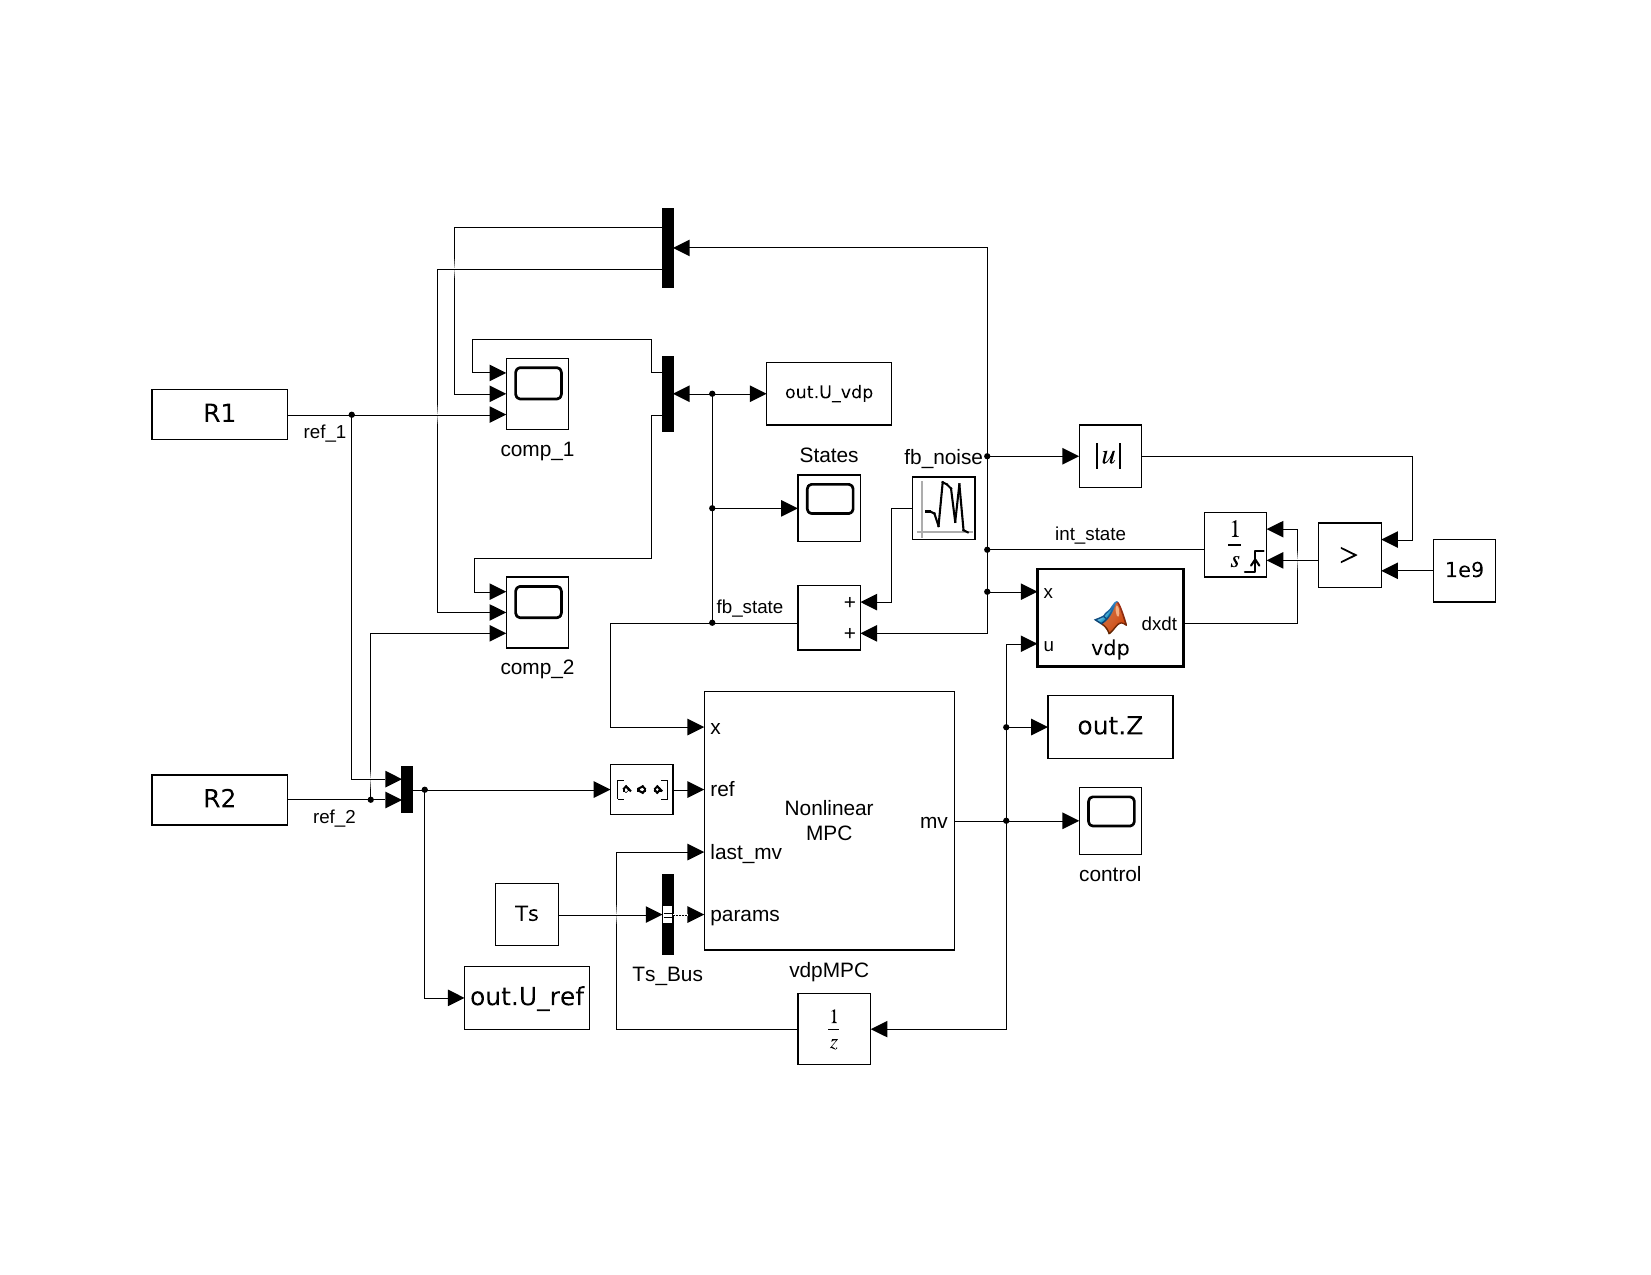
\includegraphics[width=0.75\textwidth]{VDP_nonlinear.png}
    \end{figure}
\end{frame}

\begin{frame}{Simulink model - Relevant elements}
    \small
    \begin{itemize}
        \item The Van Der Pol oscillator is implemented by using an integrator block over the output of the dynamic definition and feeding the result back to its own input. An external reset based on the absolute value of the integrated variables is implemented to avoid overflow.
        \item The nonlinear MPC requires its last output to be fed back manually; according to the documentation, this is to provide the system with the actual control signal sent to the system instead of the proposed one (for example, when using an external trim instead of bounding the minimization problem).
        \item Gaussian noise is added to the states fed back to the controller, so that real measuring conditions can be simulated. Both the noiseless internal state and the fed-back state are visually compared against the reference signal, but only the noisy signal is exported.
    \end{itemize}

    Given the length of the simulation, figures of the results are shown along with the benchmark of the Koopman operator over a shorter time-span.
\end{frame}


\section{Koopman operator}

\begin{frame}[allowframebreaks]{Observable parameters}
    For all of the koopmanized controllers, the chosen number of centroids was the highest amount that didn't yield super-unitary eigenvalues without regularization. Then, a regularization coefficient of $\num{1e-3}$ was used to obtain the definitive Koopman controller (if once regularized the eigenvalues were super-unitary, the centroid number was once again reduced).

    Additionally, a second strategy using the difference between the reference and measured states rather than the states themselves was also considered.

    \begin{itemize}
        \item Balanced controller:
            \begin{itemize}
                \item Direct: 5
                \item Differential: 12
            \end{itemize}
        \item First-state controller (only half the dataset could be used reliably):
            \begin{itemize}
                \item Direct: 26
                \item Differential: 28
            \end{itemize}
        \item Second-state controller (only a twentieth of the dataset could be used reliably)
            \begin{itemize}
                \item Direct: 18
                \item Differential: 20
            \end{itemize}
    \end{itemize}

    The output matrix \textit{C} was set to return the original control signal instead of the full-observable identity matrix, but the initial state vector has to be coherent with the observable function and the provided centroids.
\end{frame}


\section{Benchmarks}

\begin{frame}{Simulink model}
    \begin{figure}
        \centering
        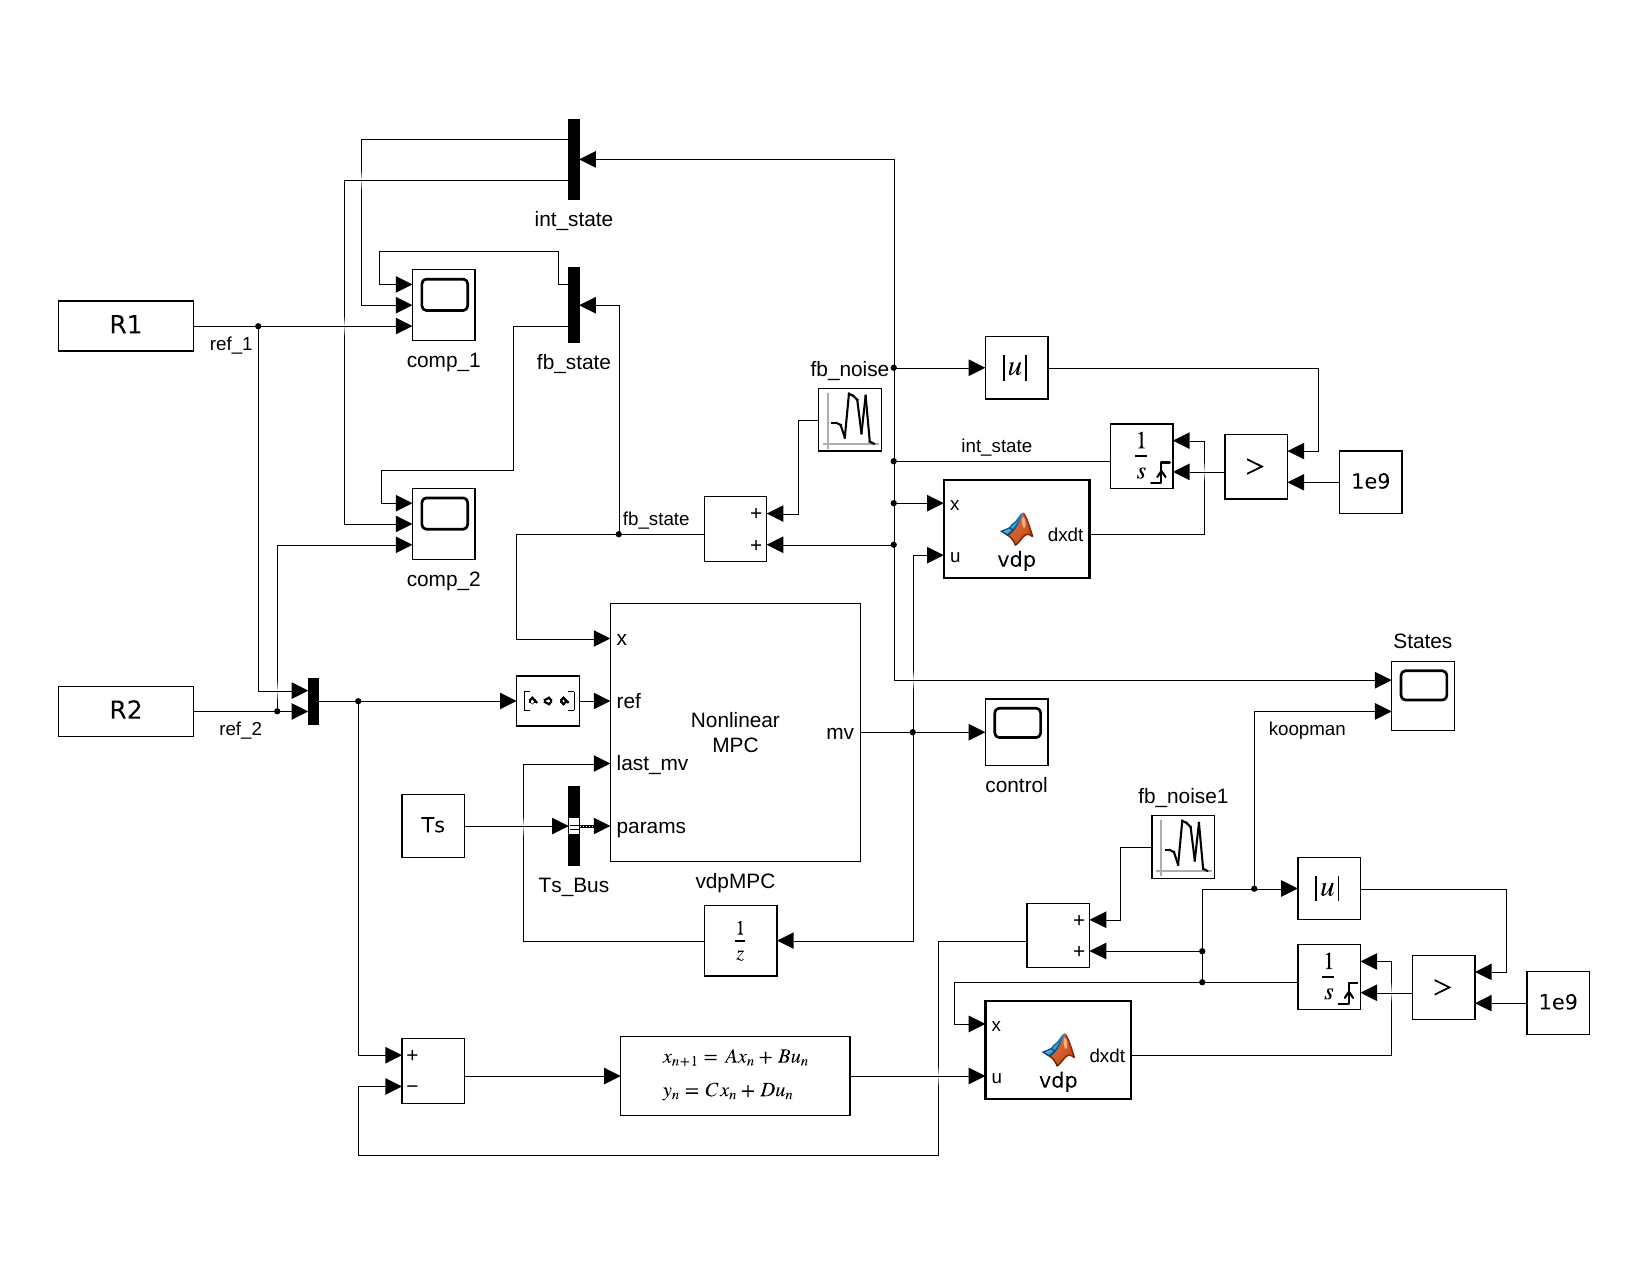
\includegraphics[width=0.75\textwidth]{VDP_comparison.png}
    \end{figure}
\end{frame}

\begin{frame}{MPC - balanced}
    \begin{figure}
        \centering
        \begin{subfigure}[b]{0.45\textwidth}
            \centering
            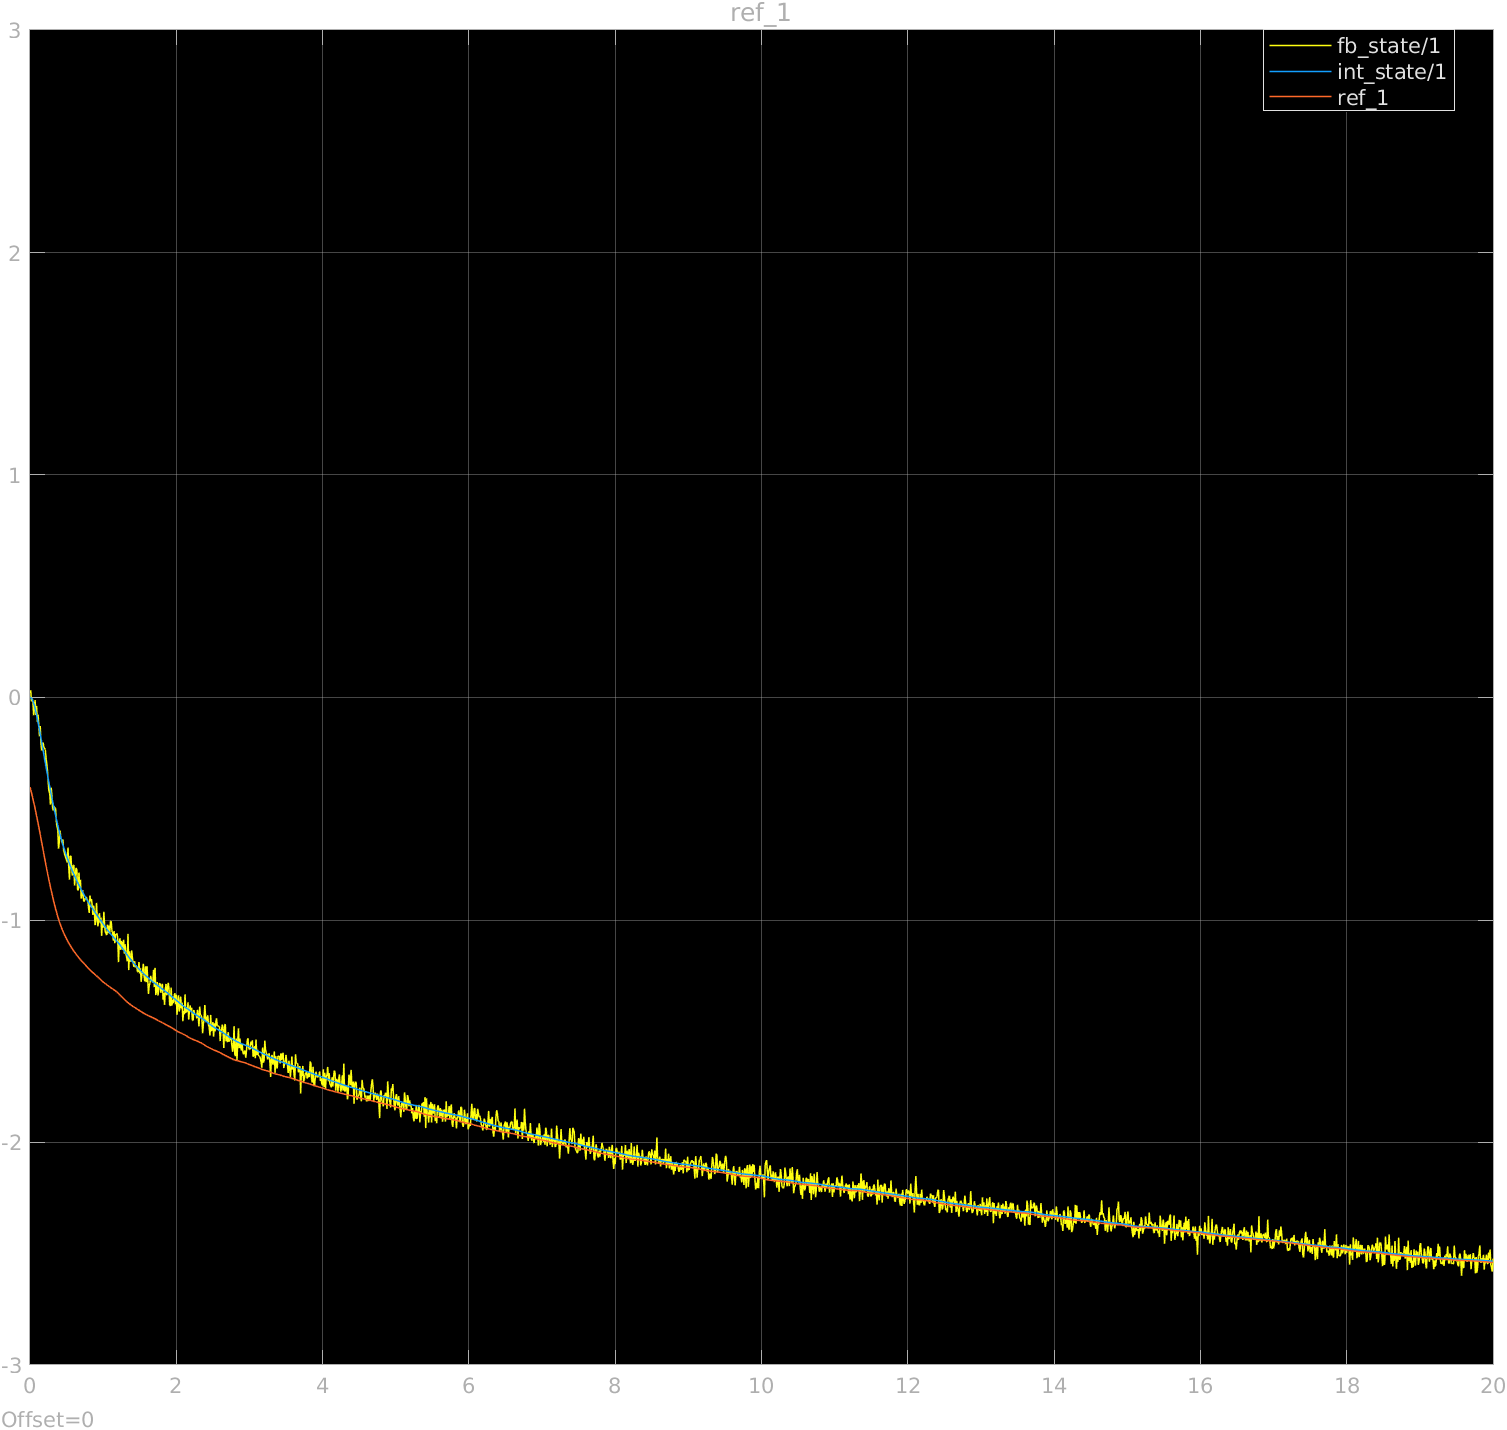
\includegraphics[width=\textwidth]{balanced_mpc_1.png}
            \caption{First state}
        \end{subfigure}
        \hfill
        \begin{subfigure}[b]{0.45\textwidth}
            \centering
            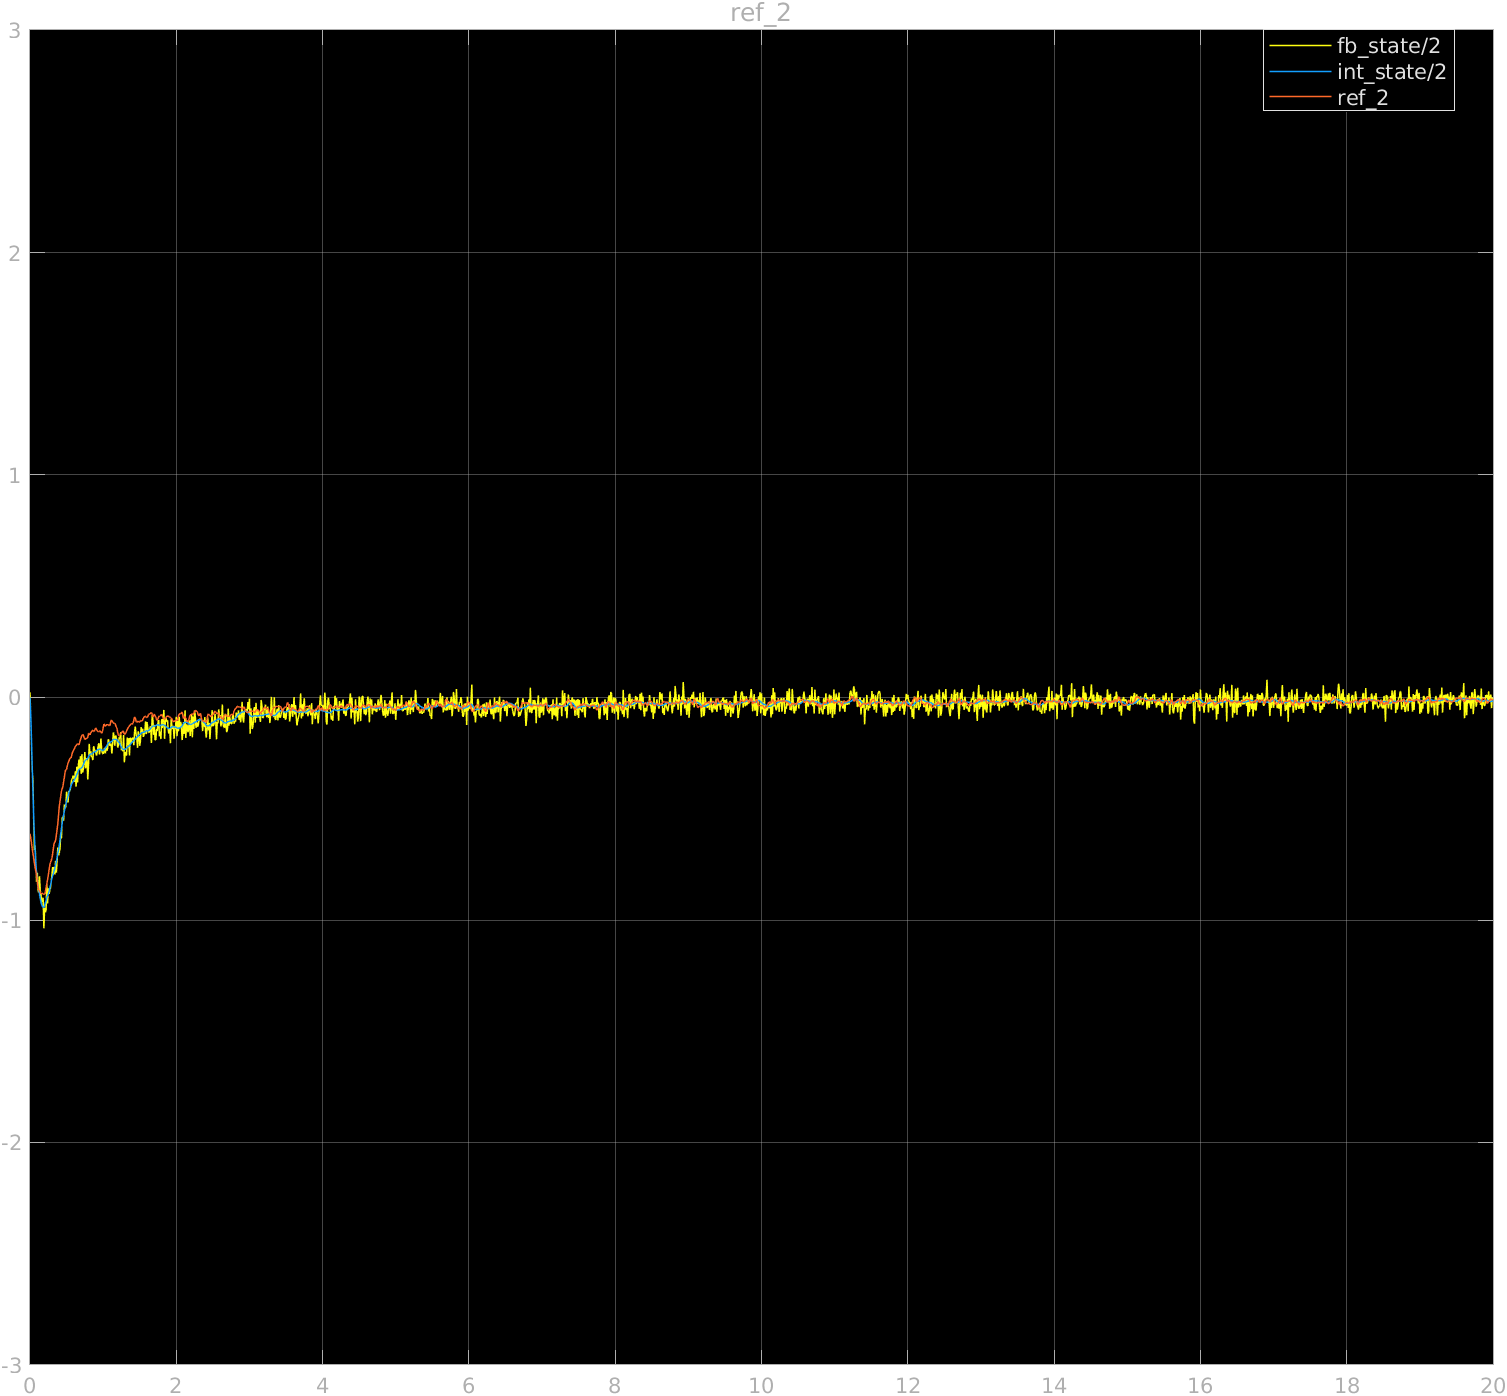
\includegraphics[width=\textwidth]{balanced_mpc_2.png}
            \caption{Second state}
        \end{subfigure}
    \end{figure}
\end{frame}

\begin{frame}{Koopman - balanced}
    \begin{figure}
        \centering
        \begin{subfigure}[b]{0.45\textwidth}
            \centering
            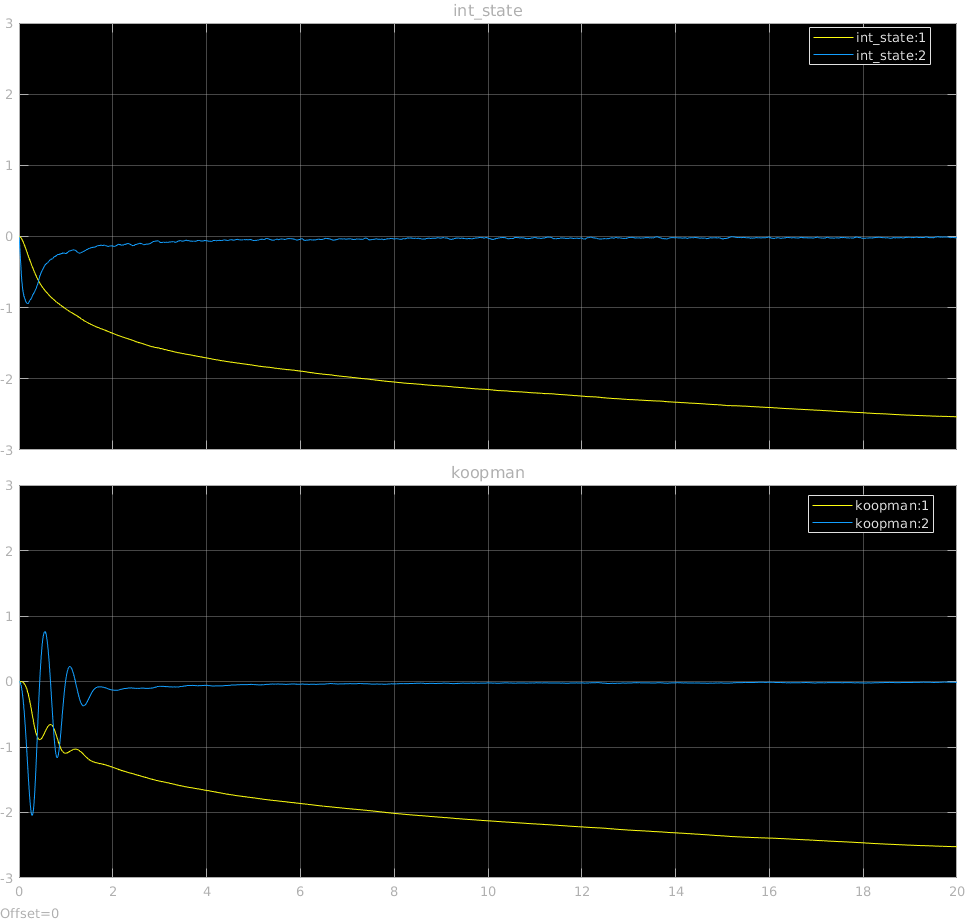
\includegraphics[width=\textwidth]{balanced_koopman_direct.png}
            \caption{Direct implementation}
        \end{subfigure}
        \hfill
        \begin{subfigure}[b]{0.45\textwidth}
            \centering
            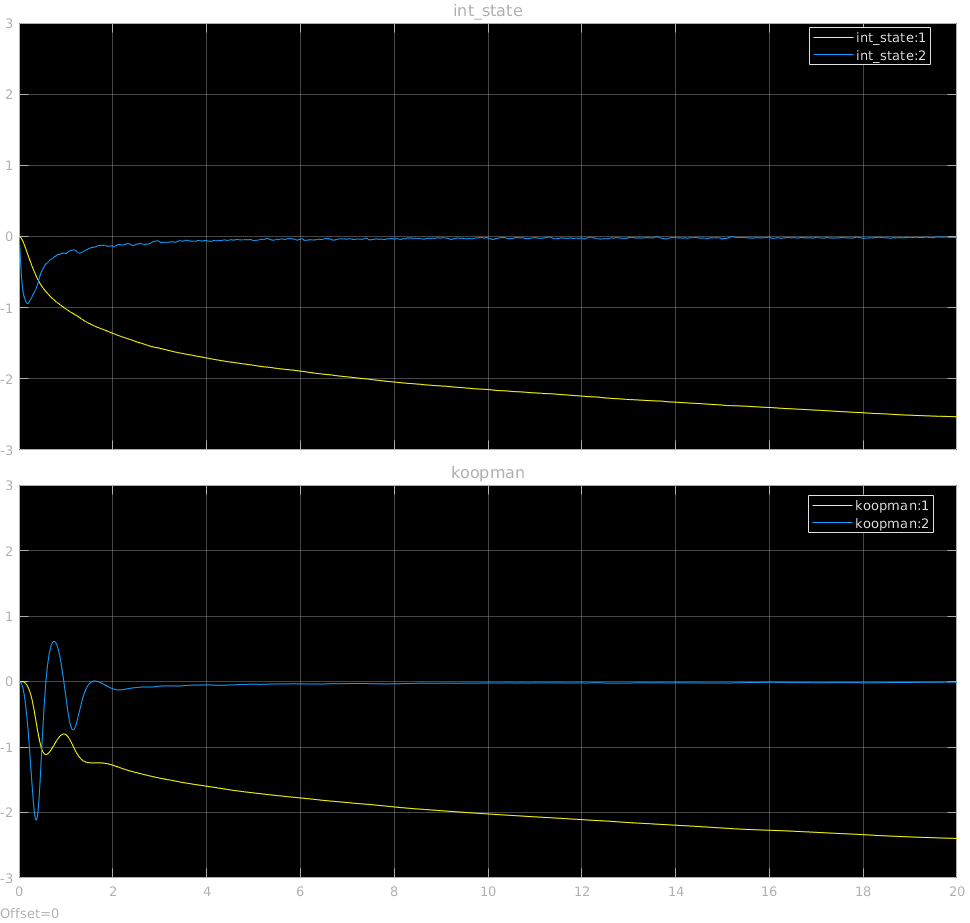
\includegraphics[width=\textwidth]{balanced_koopman_differential.png}
            \caption{Differential implementation}
        \end{subfigure}
    \end{figure}
\end{frame}

\begin{frame}{MPC - first-state}
    \begin{figure}
        \centering
        \begin{subfigure}[b]{0.45\textwidth}
            \centering
            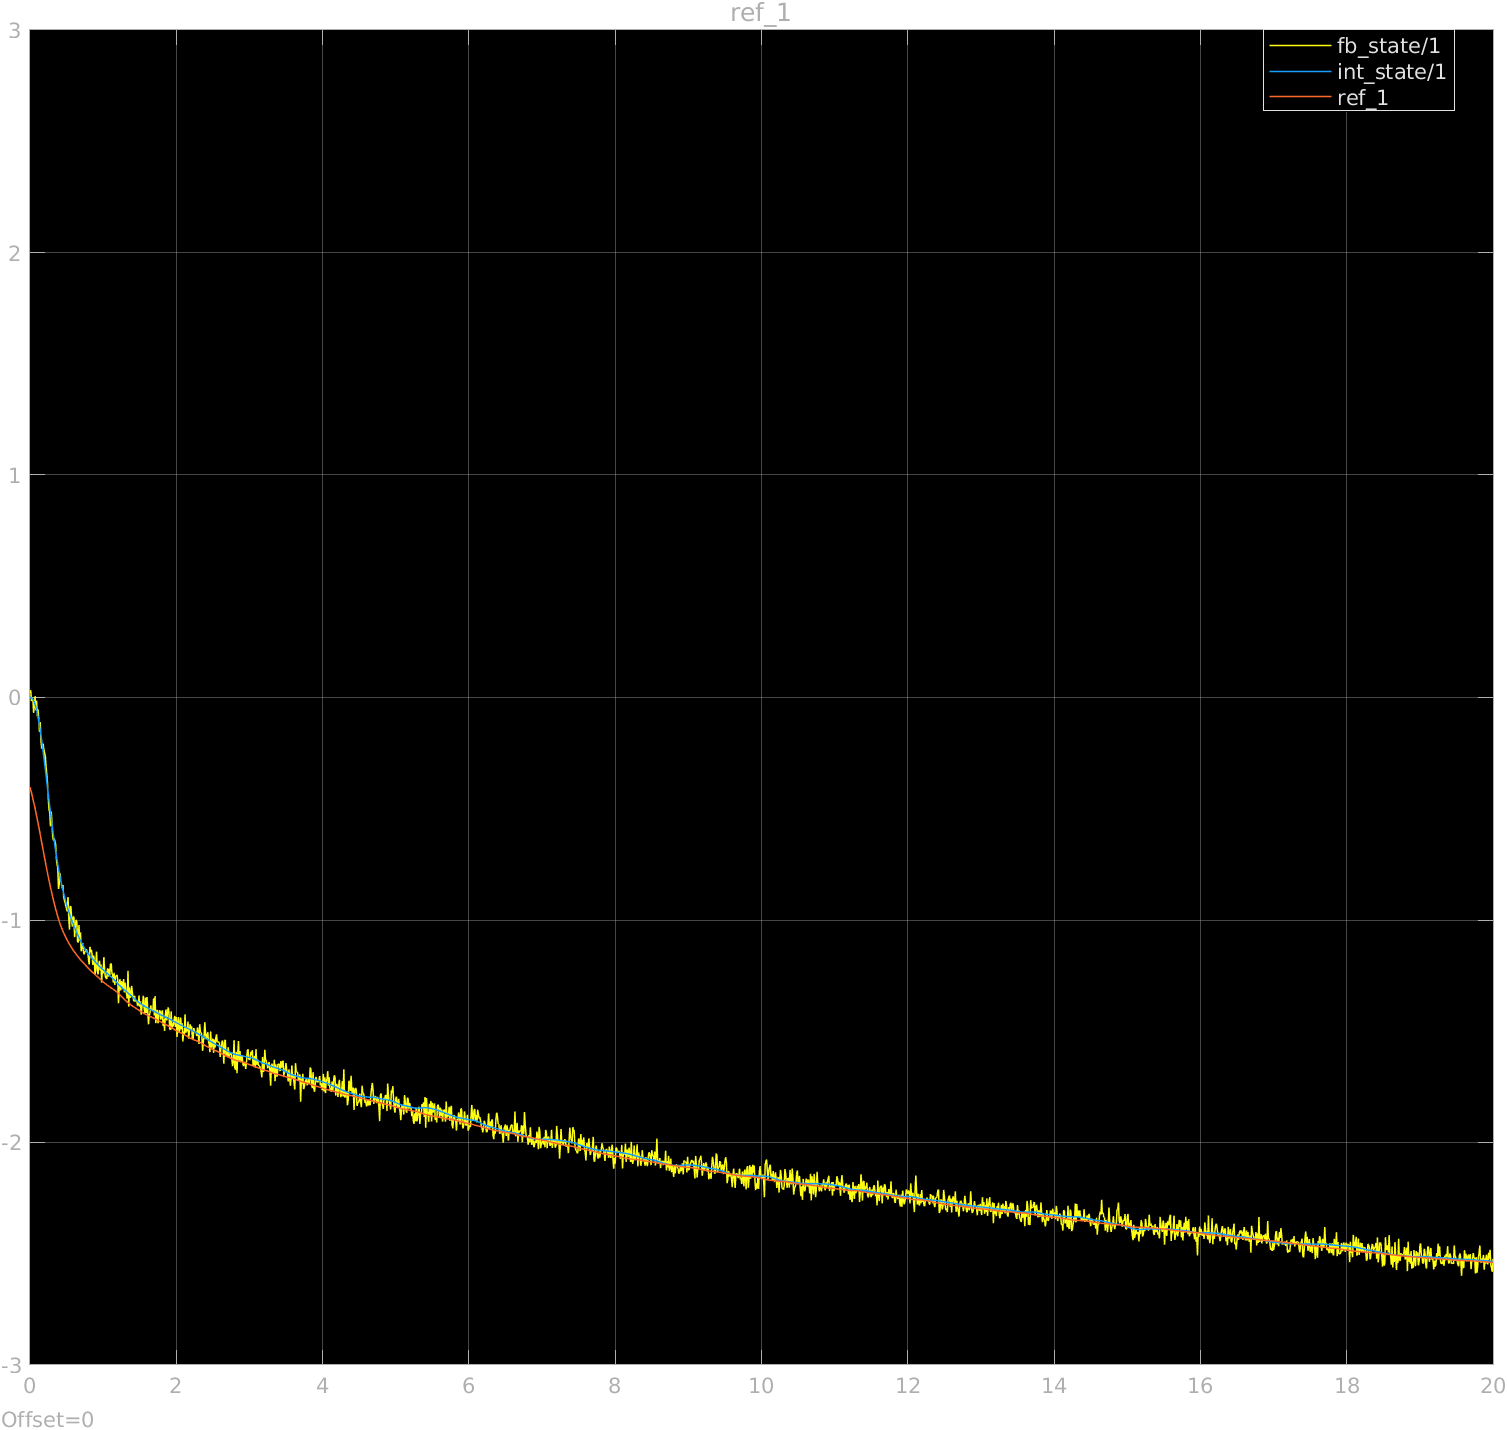
\includegraphics[width=\textwidth]{first_mpc_1.png}
            \caption{First state}
        \end{subfigure}
        \hfill
        \begin{subfigure}[b]{0.45\textwidth}
            \centering
            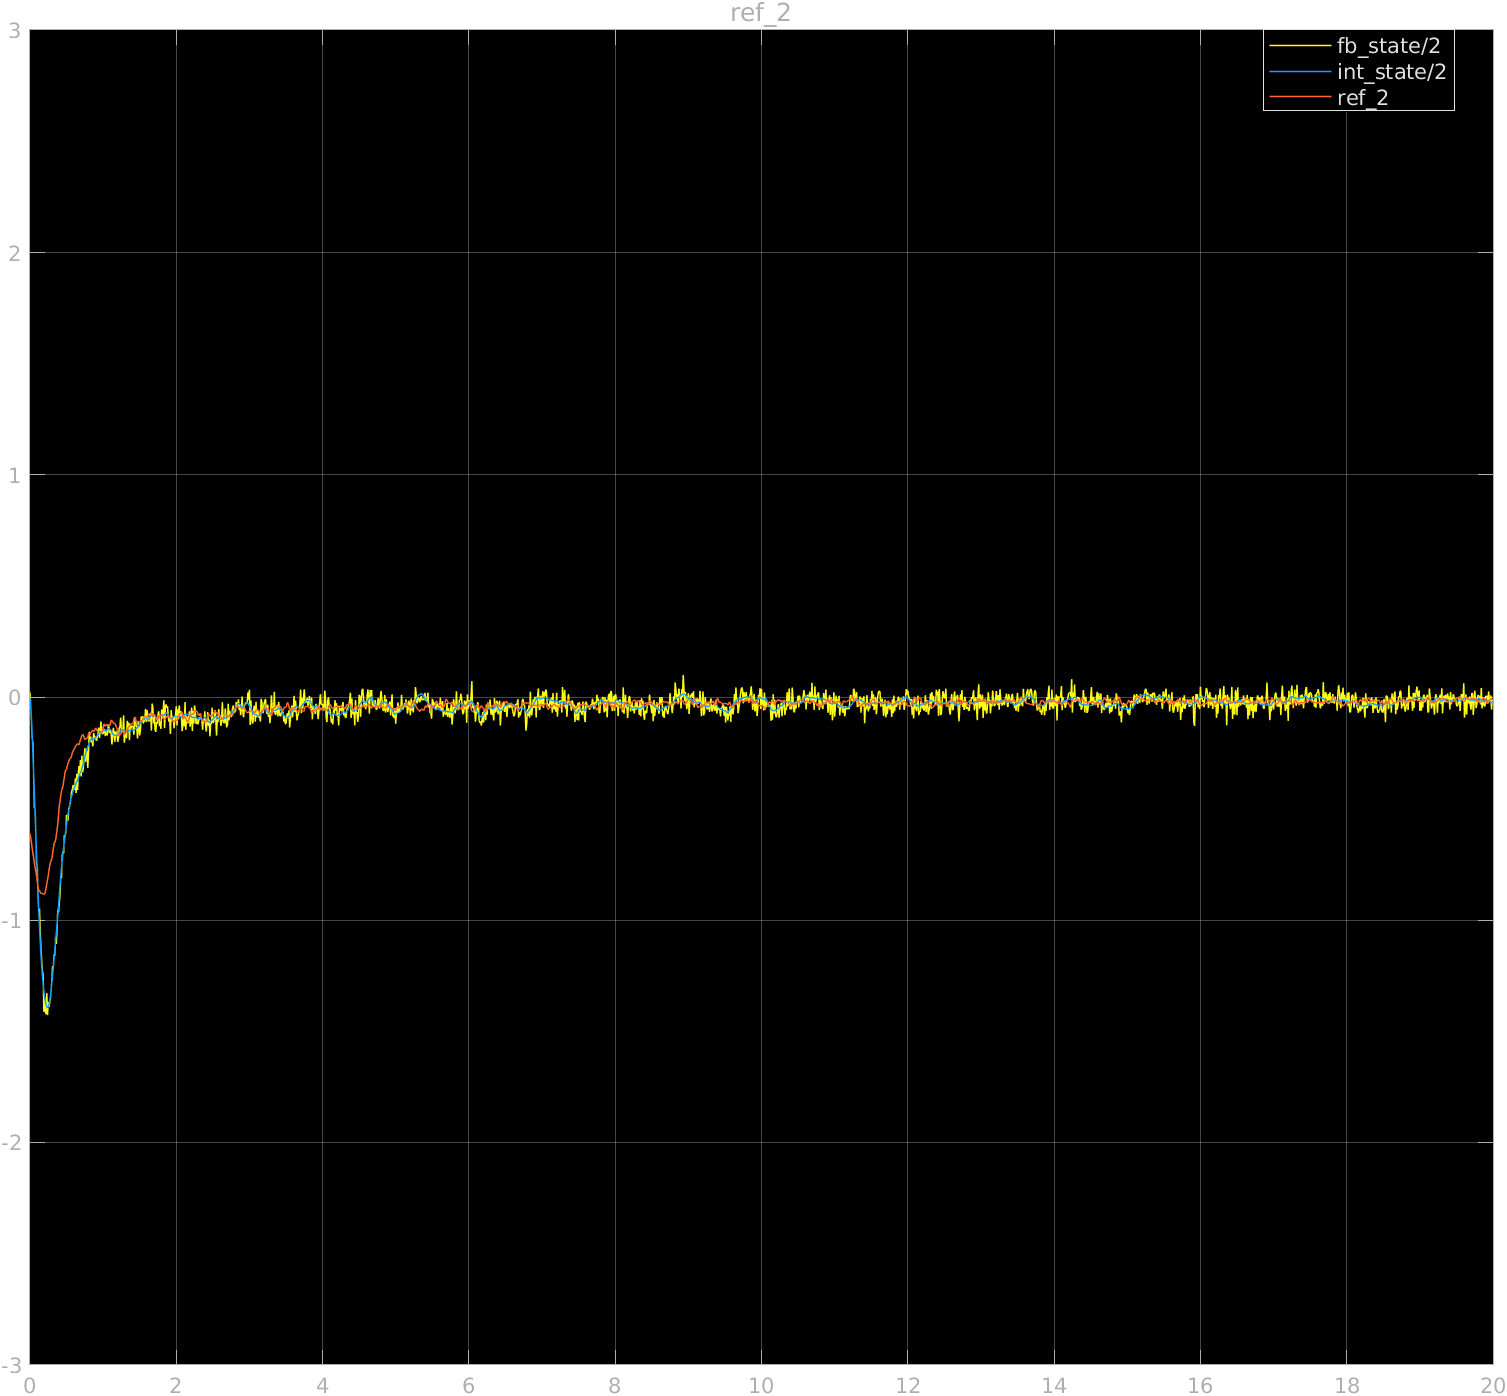
\includegraphics[width=\textwidth]{first_mpc_2.png}
            \caption{Second state}
        \end{subfigure}
    \end{figure}
\end{frame}

\begin{frame}{Koopman - first-state}
    \begin{figure}
        \centering
        \begin{subfigure}[b]{0.45\textwidth}
            \centering
            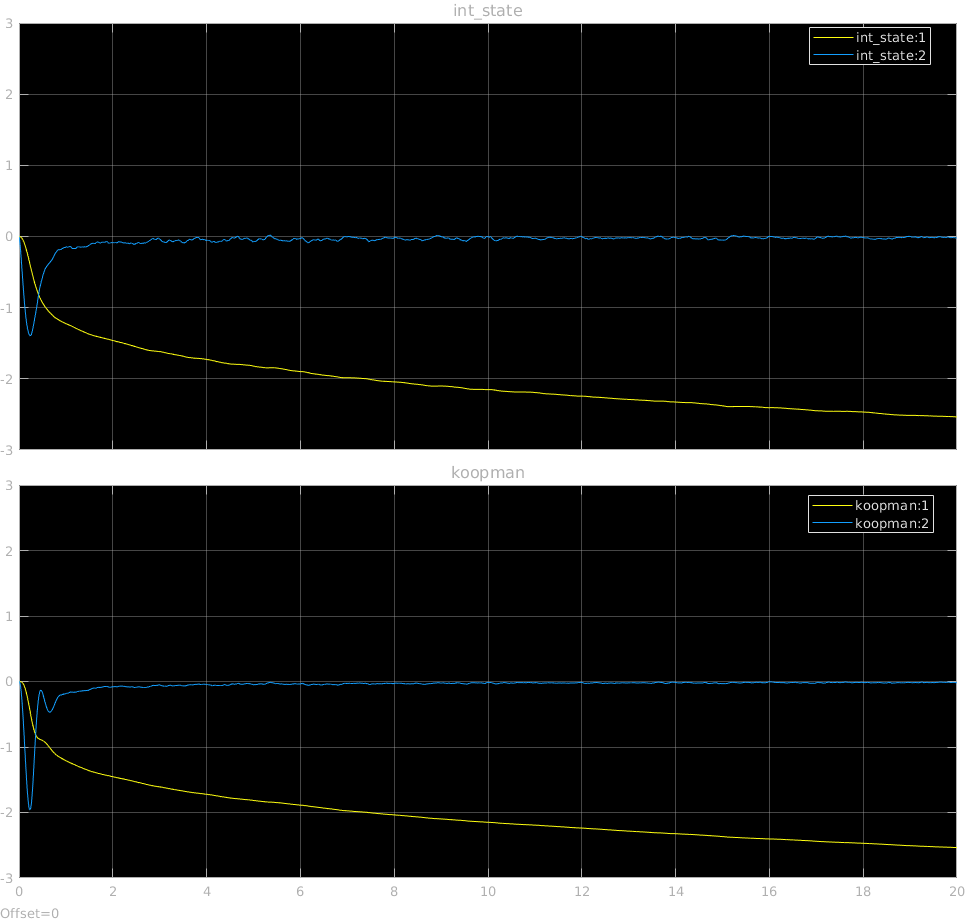
\includegraphics[width=\textwidth]{first_koopman_direct.png}
            \caption{Direct implementation}
        \end{subfigure}
        \hfill
        \begin{subfigure}[b]{0.45\textwidth}
            \centering
            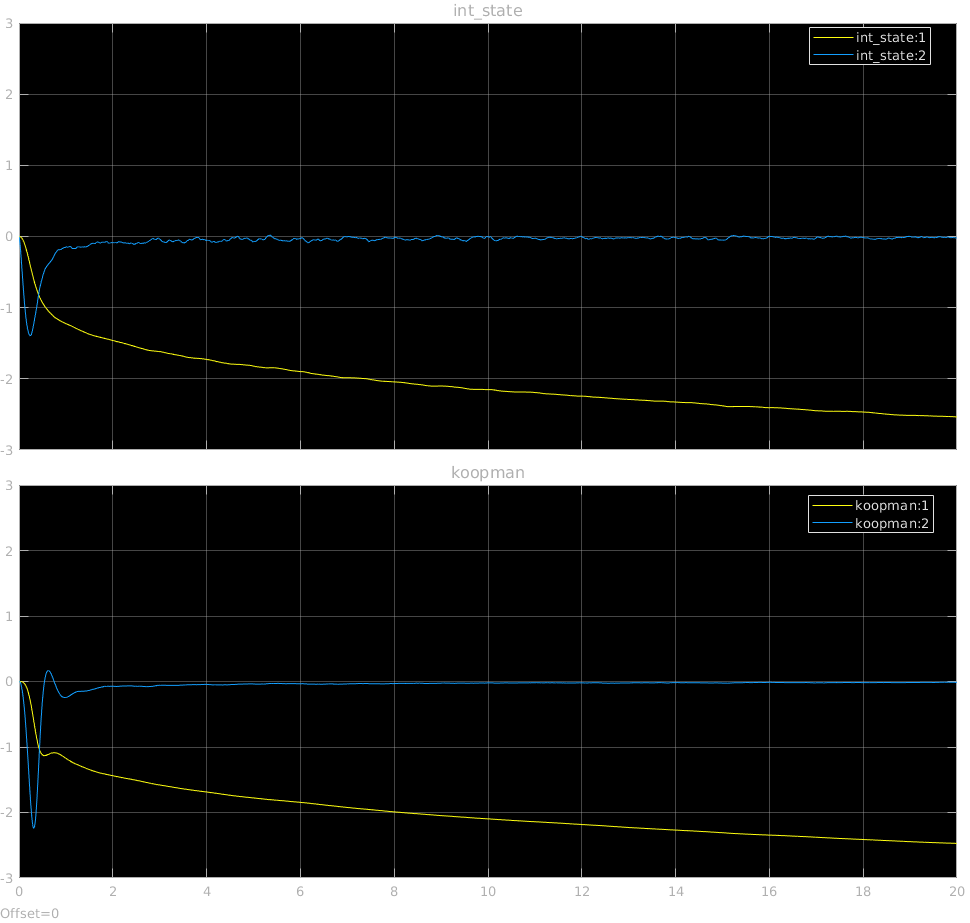
\includegraphics[width=\textwidth]{first_koopman_differential.png}
            \caption{Differential implementation}
        \end{subfigure}
    \end{figure}
\end{frame}

\begin{frame}{MPC - second-state}
    \begin{figure}
        \centering
        \begin{subfigure}[b]{0.45\textwidth}
            \centering
            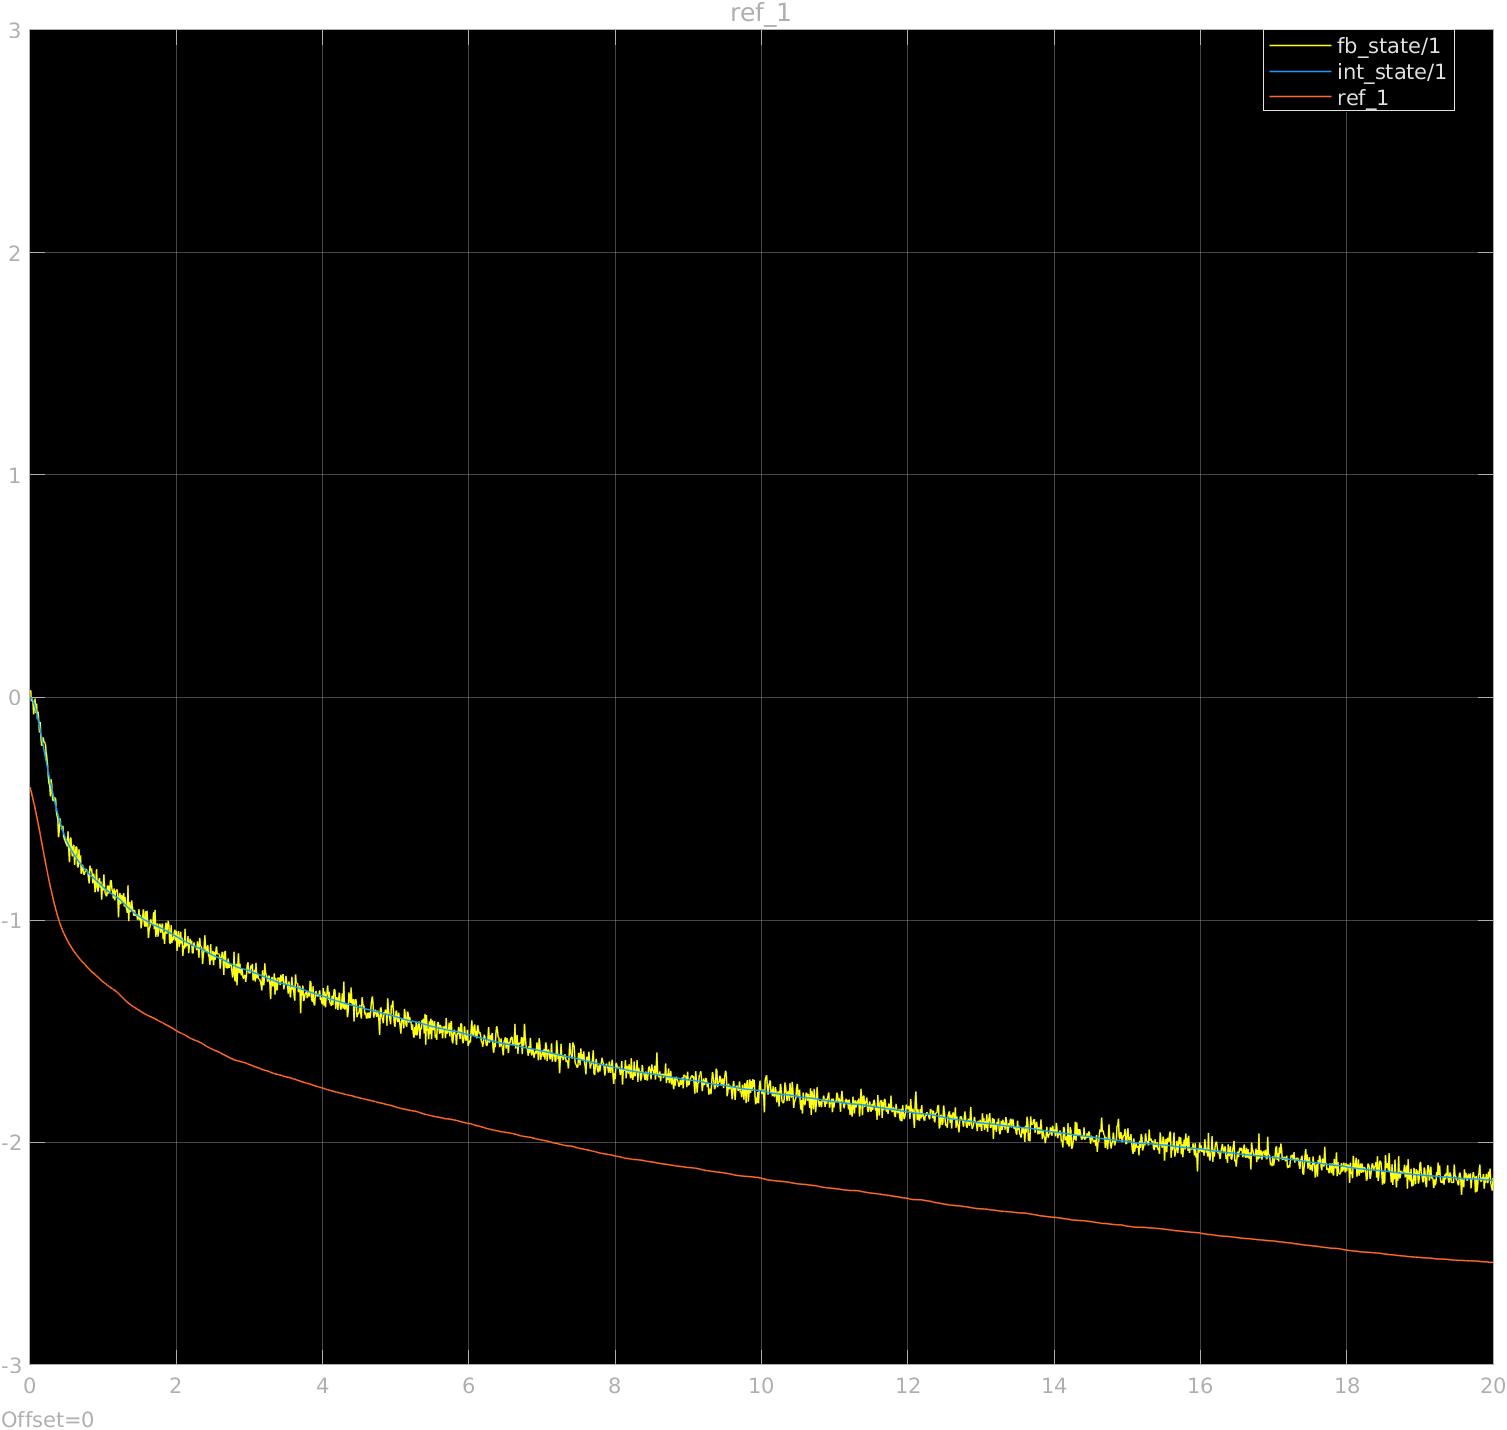
\includegraphics[width=\textwidth]{second_mpc_1.png}
            \caption{First state}
        \end{subfigure}
        \hfill
        \begin{subfigure}[b]{0.45\textwidth}
            \centering
            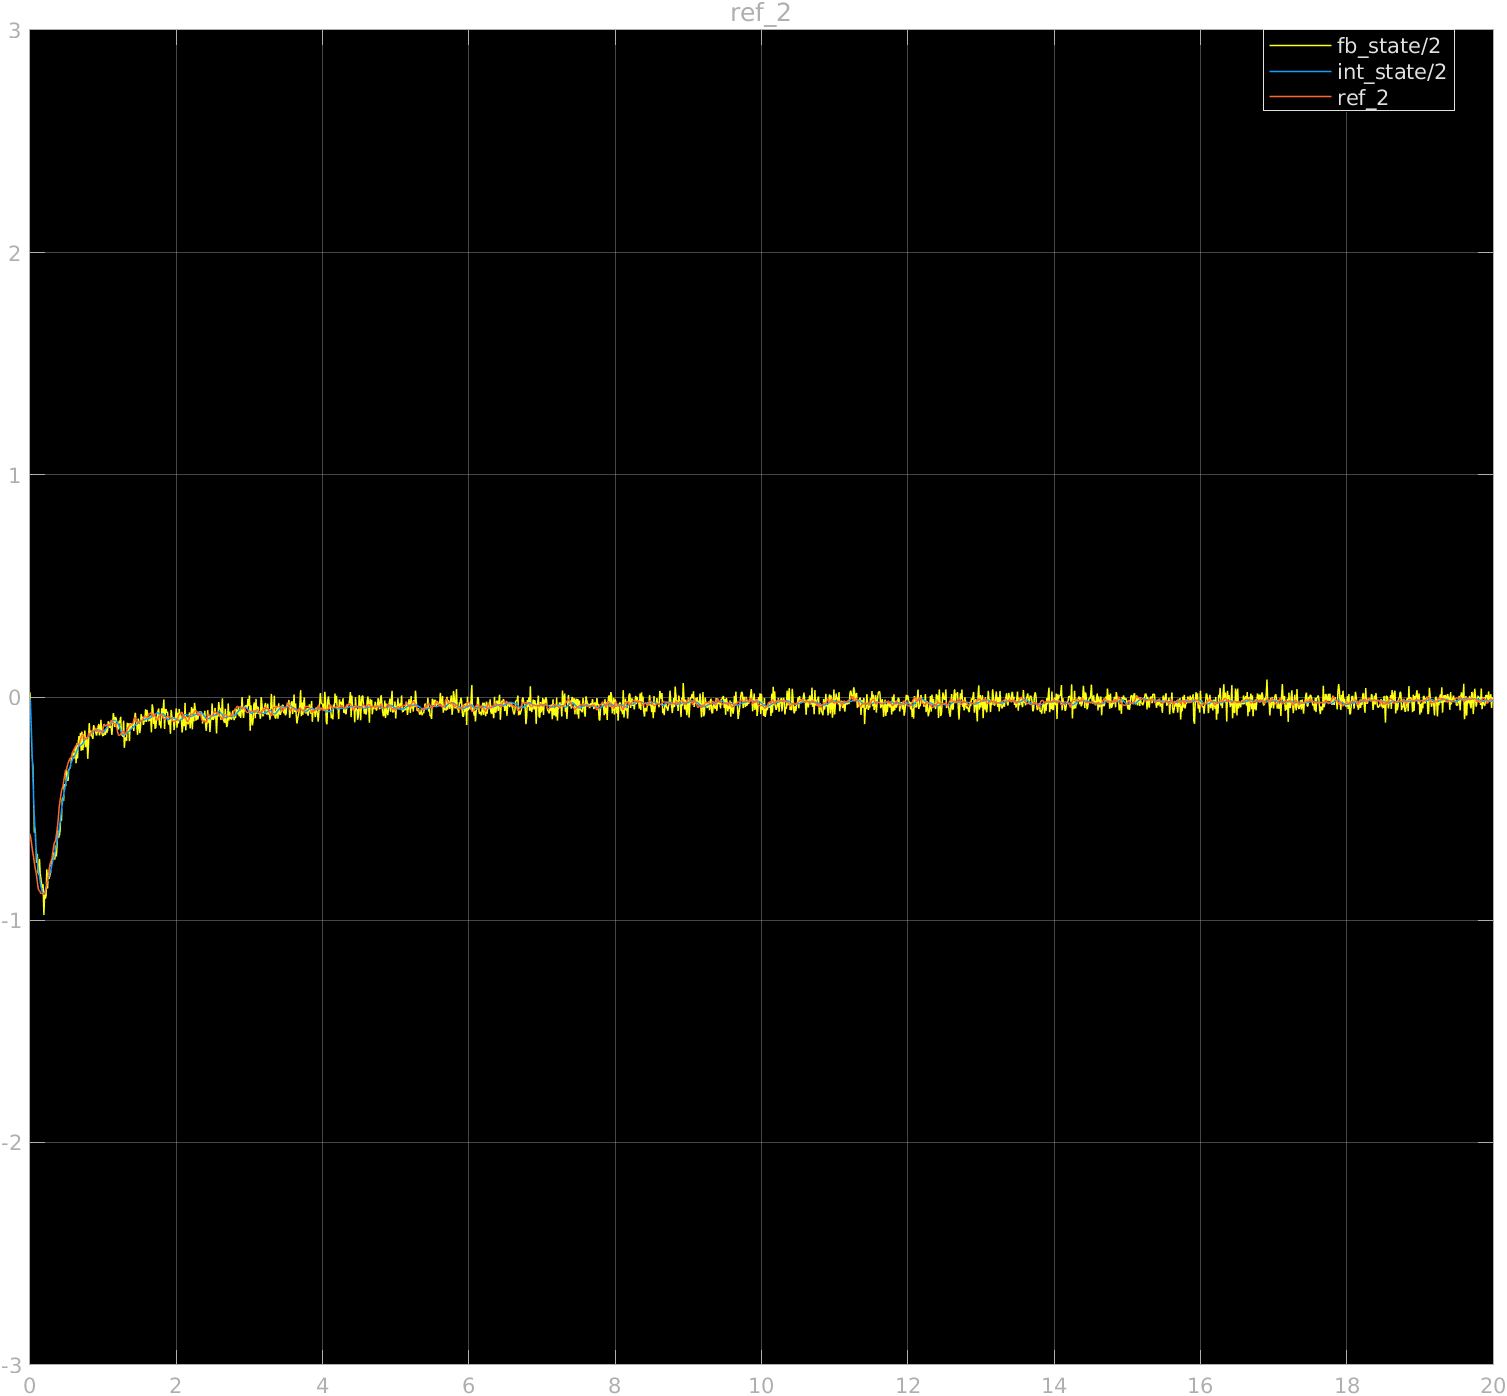
\includegraphics[width=\textwidth]{second_mpc_2.png}
            \caption{Second state}
        \end{subfigure}
    \end{figure}
\end{frame}

\begin{frame}{Koopman - second-state}
    \begin{figure}
        \centering
        \begin{subfigure}[b]{0.45\textwidth}
            \centering
            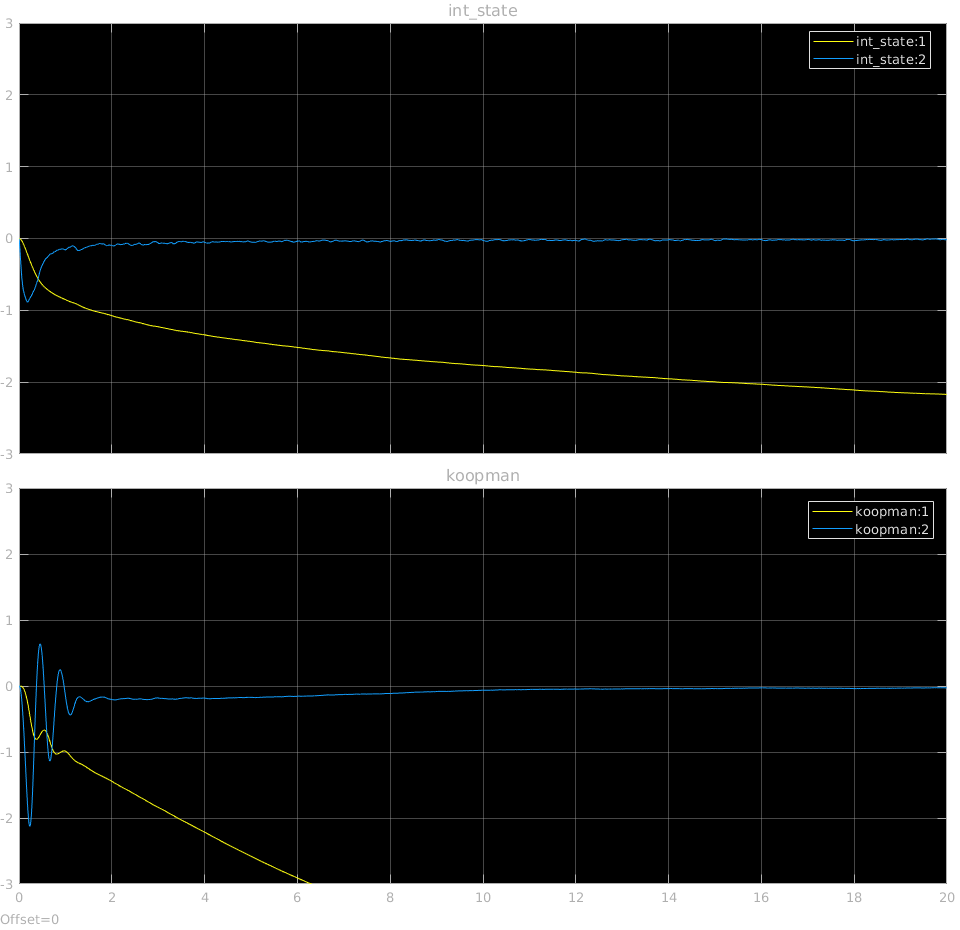
\includegraphics[width=\textwidth]{second_koopman_direct.png}
            \caption{Direct implementation}
        \end{subfigure}
        \hfill
        \begin{subfigure}[b]{0.45\textwidth}
            \centering
            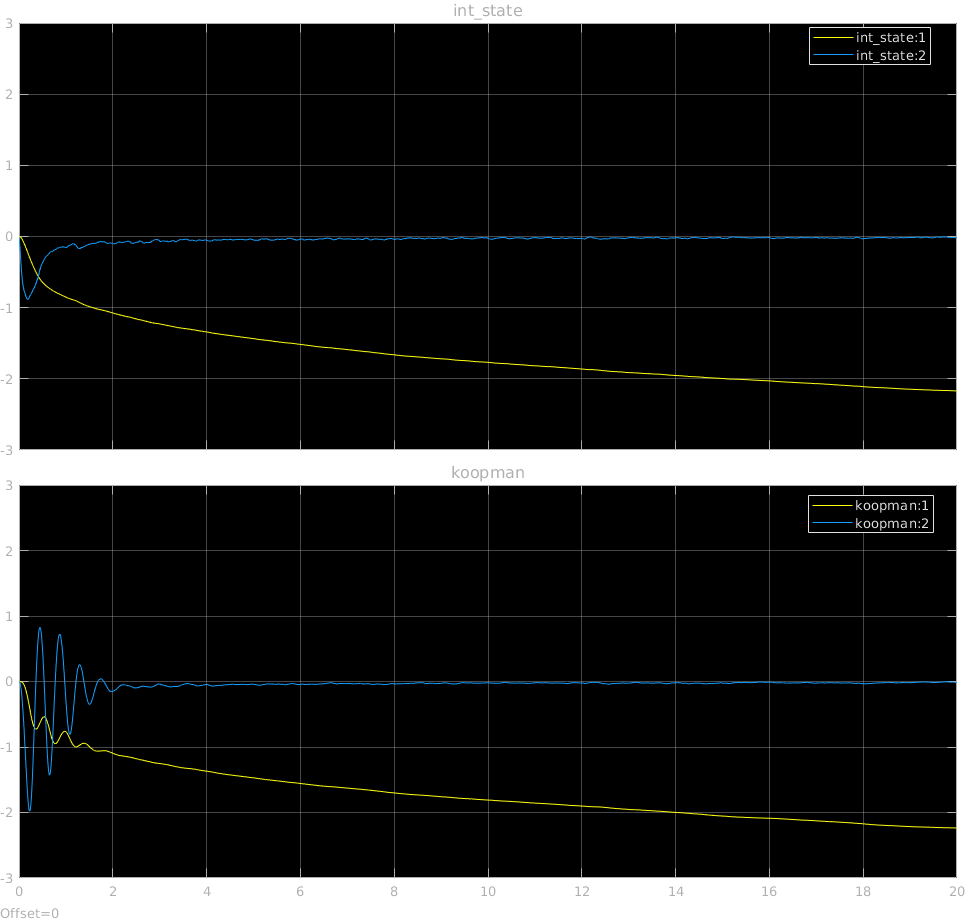
\includegraphics[width=\textwidth]{second_koopman_differential.png}
            \caption{Differential implementation}
        \end{subfigure}
    \end{figure}
\end{frame}


\section{Conclusions}

\begin{frame}[allowframebreaks]{Conclusions}
    \begin{itemize}
        \item Controlling only the second state is out of the question: even the original nonlinear MPC becomes incredibly unstable because of the second-state offset integration, which is reflected by the Koopman algorithm not being able to use more than 100 seconds (out of the 2000 simulated seconds) as valid data.
        \item Considering that we have a single input, a realistic approach is to control only the first state and recover the corresponding second state by a finite difference approach, which is reflected by the lower state overshoots and higher valid observable count. This, however, is not a realistic approach in a real-life scenario where we don't have full access to the definition of the system dynamics, making it necessary to revisit this issue down the line.
        \item In the first-state Koopman operator, the direct implementation yields a more stable result; on the other 2 controllers however, this trend is reversed, which makes theoretical sense considering the controller tries to minimize the weighed difference. An interesting alternative would be to feed both the values of the states and the difference to the Koopman algorithm (which will be considered once the design parameters for the reference nonlinear MPC are narrowed down).
    \end{itemize}
\end{frame}

\end{document}